% Preamble
\documentclass[xcolor=dvipsnames]{beamer}
\usetheme{madrid}

% Packages
\usepackage[english,ngerman]{babel}
\usepackage[utf8]{inputenc}
\usepackage{amsmath}
\usepackage{graphicx}
\usepackage{ifthen} % Boolean variables
\usepackage{subfigure} % Horizontal pictures

\definecolor{hBlue}{RGB}{55,118,165}
\usecolortheme[named=hBlue]{structure}

% Distiction between work and stream presentation
\newboolean{work}
\setboolean{work}{false}

\ifthenelse{\boolean{work}}{
    \titlegraphic{
\includegraphics[width=4cm]{../images/logo.png}}
}{}
\title{Gesundheit \& Ernährung}
\subtitle{Makronährstoffe III: Eiweiß}
\ifthenelse{\boolean{work}}{
    \author{Adrian Helberg}
}{
    \author{Bl1nzlar, twitch.tv/bl1nzlar}
}
\date{14.07.2021}


% Document
\begin{document}

    \maketitle

    \frame{\frametitle{Agenda}\tableofcontents}

    \section{Theorie}
    {
    \setbeamercolor{normal text}{fg=hBlue}\usebeamercolor*{normal text}
    \begin{frame}
        \begin{center}
            \Huge Theorie
        \end{center}
    \end{frame}
    }

    \subsection{Profil}
    \begin{frame}[allowframebreaks]
        \frametitle{Eiweiß im Profil}

        \begin{block}{Was ist Eiweiß?}
            \begin{itemize}
                \setlength\itemsep{1em}
                \item Fachwort: Protein, bei $>$ 100 Aminosäuren spricht man von Eiweiß
                \item Aminosäuren als kleinste Bausteine von Einweiß
                \item Liefert das "`Baumaterial"' für den Körper
                \item Kann bei Bedarf in Energie verbrannt werden (4 kcal/g)
                \item Ca. 20\% der Körpermasse
                \item Über 50.000 verschiedene Eiweiße im Körper aus 20 Aminosäuren
                \item 9 der 20 Aminosäuren sind essenziell
            \end{itemize}
        \end{block}

        \framebreak

        \begin{figure}
            \centering
            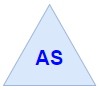
\includegraphics[width=1cm]{../images/as.png}
            \caption{Aminosäure}
        \end{figure}

        \begin{figure}
            \centering
            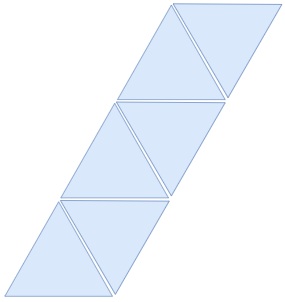
\includegraphics[width=2cm]{../images/as1.png}
            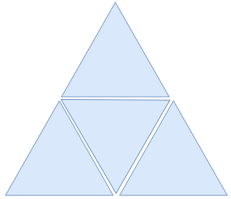
\includegraphics[width=2cm]{../images/as2.png}
            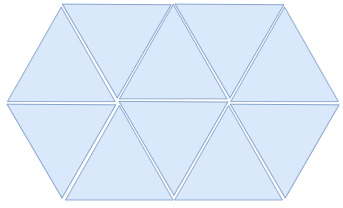
\includegraphics[width=2cm]{../images/as3.png}
            \caption{Verschiedene Kombinationen aus Aminosäuren}
        \end{figure}
    \end{frame}

    \subsection{Stoffwechsel}
    \begin{frame}[allowframebreaks]
        \frametitle{Eiweißstoffwechsel}

        \begin{itemize}
            \setlength\itemsep{1em}
            \item Eine durchschnittliche Ernährung besteht zu 15\% aus Eiweiß (ca. 75g)
            \item Ca. 70g Eiweiß wird zusätzlich aus abgestorbenen Zellen recycelt
            \item Ca. 15g Eiweiß ist schließlich Verdauungsverlust
            \item Eiweiße werden mithilfe von Verdauungsenzyme im Darm in ihre Einzelteile zerlegt
            \item Die Aminosäuren können dann die Darmwand passieren und somit ins Blut gelangen
        \end{itemize}

        \framebreak

        \begin{figure}
            \centering
            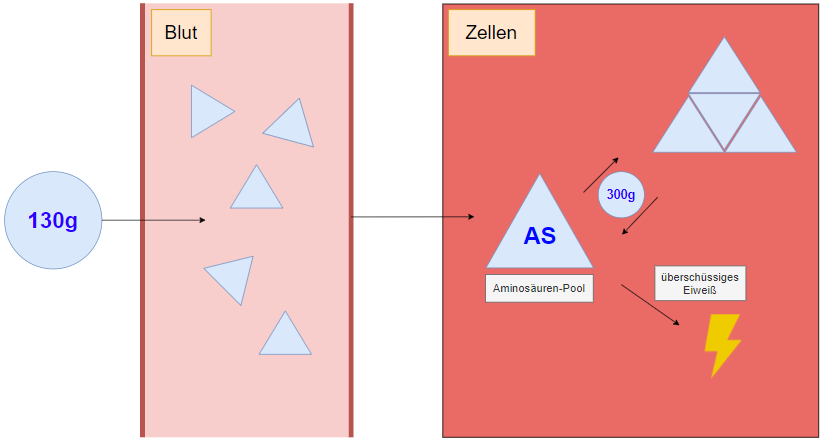
\includegraphics[width=8cm]{../images/as_stoffwechsel.png}
            \caption{Eiweißstoffwechsel Zellen}
        \end{figure}

        \framebreak

        \begin{figure}
            \centering
            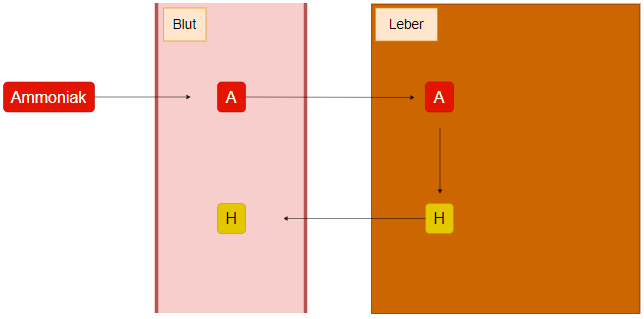
\includegraphics[width=8cm]{../images/as_stoffwechsel1.png}
            \caption{Eiweißstoffwechsel Leber}
        \end{figure}

    \end{frame}

    \subsection{Qualität}
    \begin{frame}[allowframebreaks]
        \frametitle{Eiweißqualität}

        \begin{block}{Die biologische Wertigkeit \ldots}
            \begin{itemize}
                \setlength\itemsep{1em}
                \item ist eine Methode zur Bewertung der Eiweißqualität
                \item wird durch die Zusammensetzung der Aminosäuren bestimmt
                \item referenziert das Hühnerei (Wertigkeit 100), da dieses alle essentiellen Aminosäuren in einem sehr günstigen Verhältnis enthält
            \end{itemize}
        \end{block}

        \begin{figure}
            \centering
            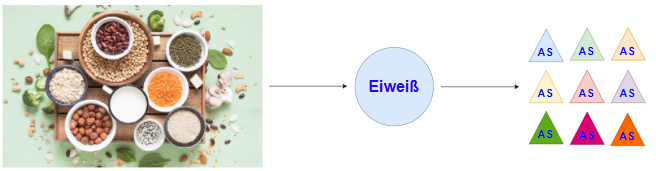
\includegraphics[width=8cm]{../images/as4.png}
            \caption{Biologische Wertigkeit von Eiweiß}
        \end{figure}

        \framebreak

        \begin{figure}
            \centering
            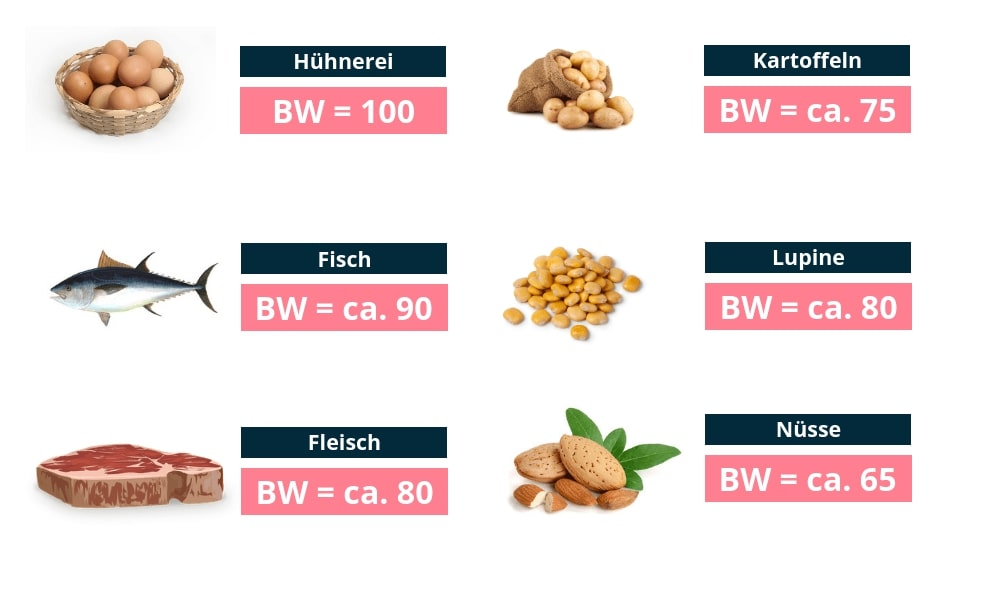
\includegraphics[width=8cm]{../images/as5.jpg}
            \caption{Biologische Wertigkeit verschiedener Lebensmitteln}
        \end{figure}

        \framebreak

        \begin{block}{Tipps für Veganer}
            \begin{itemize}
                \setlength\itemsep{1em}
                \item Hülsenfrüchte sind Pflicht!
                \item Kombinationen für eine biologische Wertigkeit von 100
                \begin{itemize}
                    \item Erbsen + Reis
                    \item Bohnen + Mais
                    \item Soja-Produkte, um die Eiweißmenge zu erhöhen
                \end{itemize}
            \end{itemize}
        \end{block}

    \end{frame}

    \subsection{Bedarf}
    \begin{frame}
        \frametitle{Bedarf}

        \begin{itemize}
            \setlength\itemsep{1em}
            \item Eiweißbedarf = Eiweißverlust aus
            \begin{itemize}
                \item Stoffwechsel $\rightarrow$ Stickstoffgehalt im Urin
                \item Verdauungsverluste $\rightarrow$ Stickstoffgehalt im Stuhl
            \end{itemize}
            \item Ein 70kg schwerer Mensch verliert ca. 24g Eiweiß am Tag
            \item[$\rightarrow$] Allgemeiner Bedarf von 0,3g / kg Körpergewicht
        \end{itemize}
    \end{frame}

    \subsection{Zufuhrempfehlung}
    \begin{frame}
        \frametitle{Zufuhrempfehlung}

        \begin{block}{Zufuhrempfehlung unter Berücksichtigung \ldots}
            \begin{itemize}
                \setlength\itemsep{1em}
                \item der Verdauungverluste (ca. 10\%) bei der Nahrungsaufnahme
                \item einer mittelmäßigen biologischen Wertigkeit
                \item eines Sicherheitszuschlages von ca. 0.5g / kg Körpergewicht
                \item[$\rightarrow$] Allgemeine Zufuhrempfehlung von 0,8g / kg Körpergewicht
                \item[$\rightarrow$] Ein 70kg schwerer Mensch sollte also 56g Eiweiß aufnehmen
            \end{itemize}
        \end{block}
        Mehrbedarf bei:
        \begin{itemize}
            \item Kindern und Jugendlichen (1g / kg Körpergewicht)
            \item Schwangerschaft (+10g EIweiß am Tag)
            \item Stillzeit (+15g Eiweiß am Tag)
            \item Leistungssportlern
        \end{itemize}
    \end{frame}

    \subsection{Sport}
    \begin{frame}[allowframebreaks]
        \frametitle{Sport}

        \begin{block}{Ausdauersport}
            \begin{itemize}
                \setlength\itemsep{1em}
                \item Leerung der Glykogenspeicher (Traubenzucker wird knapp)
                \item Traubenzucker wird im Energiestoffwechsel benötigt, also braucht der Körper eine Alternative
                \item[$\rightarrow$] Verbrennen von Aminosäuren zu Energie (Gluconeogenese)
                \item Bei Leistungssport steigt der Eiweißbedarf auf 1,2 - 1,4g / kg Körpergewicht
                \item[$\rightarrow$] Das betrifft nicht den Freizeitsportler, der 5x pro Woche Laufen geht!
            \end{itemize}
        \end{block}

        \framebreak

        \begin{block}{Kraftsport}
            \begin{itemize}
                \setlength\itemsep{1em}
                \item Eiweiß fördert den Muskelaufbau, die Leistungsfähigkiet und die Regeneration
                \item Bei Leistungssport steigt der Eiweißbedarf auf 1,6g / kg Körpergewicht
                \item Studien belegen keine weiteren Vorteile bei einer Eiweißaufnahme von über 2g / kg Körpergewicht
            \end{itemize}
        \end{block}

        \framebreak

        \begin{block}{Eiweißbedarf bei Sportlern}
            \begin{itemize}
                \setlength\itemsep{1em}
                \item Kraftsportler von 80kg
                \item Tägliche Kalorienzufuhr von 3000 kcal
                \item Eiweißanteil der Ernährung von über 20\% durch eiweißreiche Lebensmittel
                \item[$\rightarrow$] Das entspricht einer Eiweißzufuhr von 1,9g / kg Körpergewicht
            \end{itemize}
        \end{block}

        \framebreak

        \begin{block}{Ist zu viel Eiweiß schädlich?}
            \begin{itemize}
                \setlength\itemsep{1em}
                \item Bis vor kurzem: Kein wissenschaftlicher Beweis
                \item Nieren werden stärker Belastet
                \item Erhöhter Verlust von Mineralstoffen, wie zB. Calcium
                \item "`Sichere"' Obergrenze von 2g / kg Körpergewicht
            \end{itemize}
        \end{block}
    \end{frame}

    \subsection{Gluten}
    \begin{frame}[allowframebreaks]
        \frametitle{Gluten}

        \begin{block}{Gluten \ldots}
            \begin{itemize}
                \setlength\itemsep{1em}
                \item sind Klebereiweiße
                \item kommt in Weizen, Roggen und Gerste vor
                \item hält beim Brotbacken den Teig zusammen
                \item hält Luftbläschen fest, die bei der Teiggärung entstehen
            \end{itemize}
        \end{block}

        \framebreak

        \begin{block}{Probleme im Zusammenhang mit Gluten}
            \begin{itemize}
                \setlength\itemsep{1em}
                \item Gluten führt bei vielen Menschen zu einer Autoimmunreaktion des Darmes (Zöliakie)
                \item Gluten führt bei vielen Menschen zu Glutensensitivität
                \begin{itemize}
                    \item Verdauungsproblemen
                    \item Schmerzen
                    \item Migräne
                    \item Konzentrationsschwäche
                    \item Chronischer Erschöpfung
                    \item Depression
                    \item Blutarmut
                    \item Taubheitsgefühle
                \end{itemize}
                \item Gluten führt bei vielen Menschen zum "`Leaky Gut Syndrome"'
            \end{itemize}
        \end{block}

        \framebreak

        \begin{block}{Forschung}
            \begin{itemize}
                \setlength\itemsep{1em}
                \item Prof. Alessio Fasano
                \item "`Gluten ist für jeden Menschen schädlich, aber nicht jeder Mensch wird krank"'
                \item Darmspalten lassen sich öffnen und schließen, was durch Zonulin gesteuert wird
                \item Aufgrund der speziellen Struktur von Gluten haben die Verdauungsenzyme Probleme damit das
                Gluten in freie Aminosäuren zu spalten $\rightarrow$ es entstehen "`Bruchstücke"'
                \item Gedunde Menschen "`gewinnen"' den Kampf gegen die körperfremden Bruchstücke
            \end{itemize}
        \end{block}

        \framebreak

        \begin{figure}
            \centering
            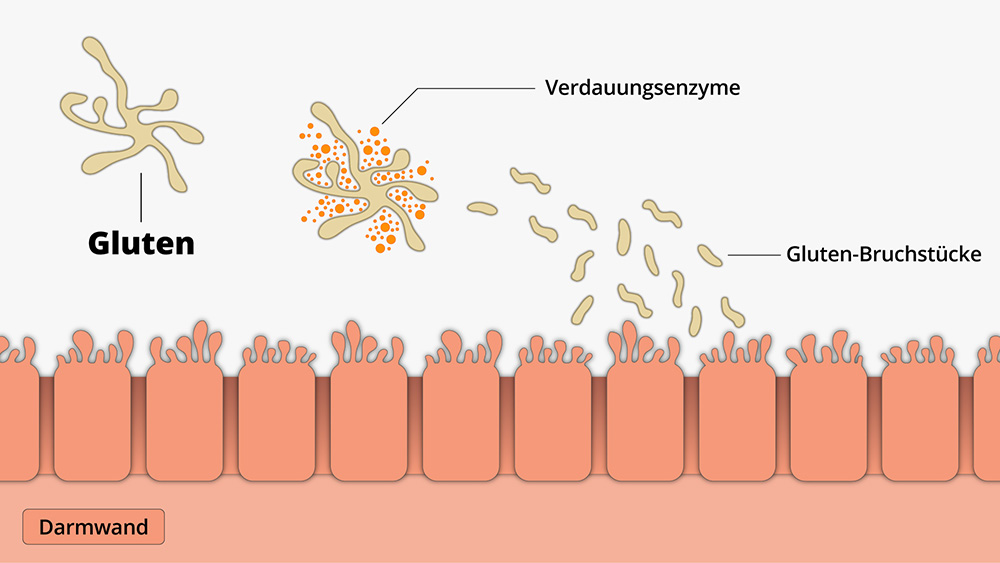
\includegraphics[width=10cm]{../images/gluten.jpg}
            \caption{Glutenverdauung}
        \end{figure}

        \framebreak

        \begin{figure}
            \centering
            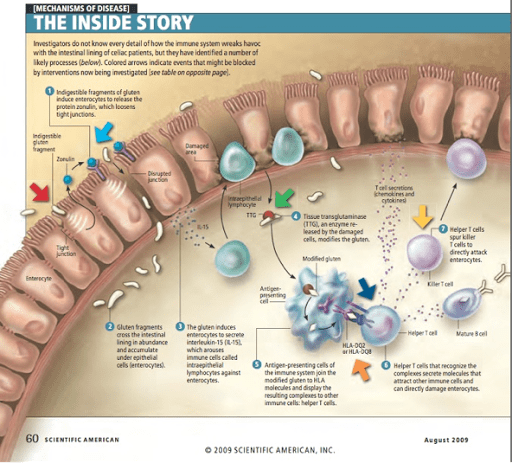
\includegraphics[width=7cm]{../images/zonulin.png}
            \caption{Zonulinausschüttung bei Glutenverdauung}
        \end{figure}
    \end{frame}

    \subsection{mTOR}
    \begin{frame}[allowframebreaks]
        \frametitle{mTOR}

        \begin{block}{\textit{Mechanistic Target of Rapamycin} \ldots}
            \begin{itemize}
                \setlength\itemsep{1em}
                \item ist ein Protein, das gezielt Moleküle "`aktiviert"'
                \item beeinflusst die Vermehrung von Zellen und die Signalkaskade einer Immunantwort
                \item wird durch Rapamycin gehemmt und wirkt dann gegenteilig
                \item[$\rightarrow$] Eine Aktivierung wirkt leistungssteigernd, wachstumsfördernd, muskelaufbauend und wundheilend
                \item[$\rightarrow$] Eine Hemmung verringert Entzündungsvorgänge und macht Autophagie (zelluläre Regenerations- und Reparationsvorgänge)\\ erst möglich
            \end{itemize}
        \end{block}

        \framebreak

        \begin{block}{Aktivierung}
            \begin{itemize}
                \setlength\itemsep{1em}
                \item Hoher Blutspiegel von essentiellen Aminosäuren
                \item Hoher Blutspiegel von Traubenzucker
                \item Hoher Insulinblutspiegel
                \item Hoher Energiestatus (ATP) in den Zellen
                \item Starker mechanischer Trainingsreiz
            \end{itemize}
        \end{block}

        \framebreak

        \begin{block}{Hemmung}
            \begin{itemize}
                \setlength\itemsep{1em}
                \item Nahrungsmangel (temporäres Fasten, da keine mTOR-Hämmung, wenn der Aminosäurenpool zu stark absinkt)
                \item Unterstützend wirken mTOR-hemmend:
                \begin{itemize}
                    \item Melatonin (Schlafhormon)
                    \item Vitamin D
                    \item Alphaliponsäure (Antioxidans)
                    \item bestimmte Polyphenole (zB. im schwarzen, ungesüßten Kaffee)
                    \item Oleocanthal und Oleuropein (zB. in Olivenöl und Olivenblattextrakt)
                \end{itemize}
            \end{itemize}
        \end{block}

        \framebreak

        \begin{block}{Fazit aus der Forschung}
            \\~\\
            \textit{"`Ein gesunder Organismus braucht sowohl mTor-Aktivierung, als auch mTor-Hemmung, idealerweise
            in natürlichen Zyklen. Ist mTor aktiviert werden Zellen aufgebaut (u.a. Muskelaufbau) und die Wundheilung
            gefördert. Eine Hemmung von mTor hingegen reduziert Entzündungen, erhöht die Reparaturvorgänge im Körper
            (Autophagie) und fördert daher auch die Langlebigkeit. Zur Optimierung der eigenen Gesundheit gilt es seinen
            praxistauglichen „Sweet-Spot“ zu finden, indem nach einer Phase der mTor-Aktivierung eine Phase der
            mTor-Hemmung folgt, beispielsweise durch die Kombination einer eiweißreichen Kost und körperlicher
            Betätigung, gefolgt von Kurzzeitfasten."'}
            \\~\\
        \end{block}
    \end{frame}

    \section{Praxis}
    {
        \setbeamercolor{normal text}{fg=hBlue}\usebeamercolor*{normal text}
        \begin{frame}
            \begin{center}
                \Huge Praxis
            \end{center}
        \end{frame}
    }

    \begin{frame}{Tipps \& Tricks}
        \begin{itemize}
            \setlength\itemsep{1em}
            \item Gluten reduzieren, zB. Backwaren (mal wieder)
            \begin{itemize}
                \item Weizen, Roggen, Gerste ("`Nur"' drei Getreidepflanzen meiden)
                \item Selbsttest: 14 Tage lang glutenfreie Ernährung
                \item Glutenbedingte Beschwerden verschwinden in kurzer Zeit und man kann dises dann auf Gluten zurückführen
            \end{itemize}
            \item Vortrag von Prof. Alessio Fasano: https://www.youtube.com/watch?v=VvfTV57iPUY
            \item Ein guter Einstieg in eine insgesamt gesündere Ernährungsweise mit dem Fokus auf natürliche, echte Lebensmittel im Vordergrund stehen
            \item Temporäres Fasten
        \end{itemize}
    \end{frame}

    \section{Fragerunde}
    {
        \setbeamercolor{normal text}{fg=hBlue}\usebeamercolor*{normal text}
        \begin{frame}
            \begin{center}
                \Huge Fragerunde
            \end{center}
        \end{frame}
    }

\end{document}